%%%%%%%%%%%%%%%%%%%%%%%%%%%%%%%%%%%%%%%%%%%%%%%%%%%%%%%%%%%%%%%%%%%%%%%%%%%
% Juan Manuel Perez Rua
%%%%%%%%%%%%%%%%%%%%%%%%%%%%%%%%%%%%%%%%%%%%%%%%%%%%%%%%%%%%%%%%%%%%%%%%%%%

\chapter{Object Flow Pipeline} \label{chap:core}

\section{Algorithm description}
\label{sec:desc}

Following the definition of the problem given in the Section \ref{sec:definition}, a 
 system for computing the object flow have devised.
The Fig. \ref{figurelabel_sys} shows a simplified block diagram of the proposed system. It is important to recognize the two main 
components of our work-flow: object tracking and segmentation, and pixel-wise flow computation on the pixels of interest.  The scheme is completed by feeding back the flow 
information to improve the tracker as depicted in the figure. For instance, one can make the most of dense displacement vectors to refine the motion of the target, and 
the segmentation information can be used to improve the sampling process of the learning stage in several trackers by detection methods \cite{c22}. Thus, 
the tracker and motion flow algorithm can work for mutual enhancement.

   \begin{figure}[thpb]
      \centering
      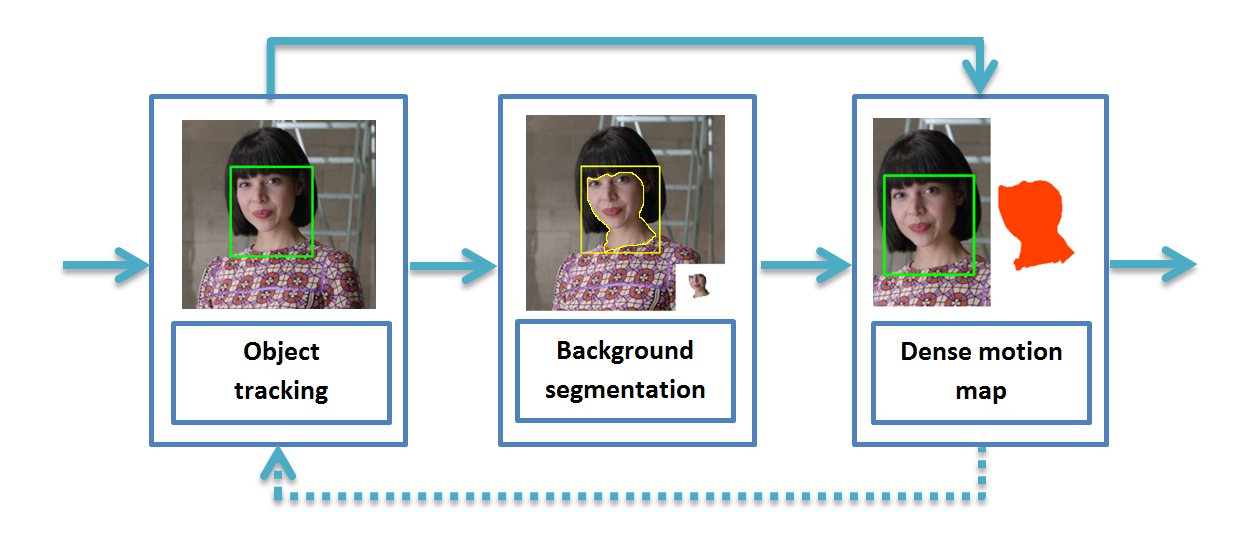
\includegraphics[width=1.00\textwidth]{../images/system.png}
      \caption{Block diagram of the proposed pipeline.}
      \label{figurelabel_sys}
   \end{figure}

 The object tracking in the object flow pipeline can be selected according to a specific need for a given application. Here, recent methods based on tracking-by-detection are preferred, given that they are in the top of modern benchmarks for object tracking \cite{c16} in terms of accuracy and stability to initialization changes. Even more, as previously mentioned 
tracking-by-detection techniques benefit from the background-foreground separation of the next stage in the object flow pipeline. For instance, the sampling process in the {\it Struck} 
tracker can be improved by selecting positive samples only inside the region of the target object.
In the second place, for the object segmentation in video, the 
labelled background regions through the concept of superpixel flow, as explained in 
Section \ref{chap:suppix}, is shown. The last step, the flow computation, uses a modified 
{\it Simple Flow} algorithm, which uses the provided segmentation masks for an accurate estimation.

%%%%%%%%%%%%%%%%%%%%%%%%%%%%%%%%%%%%%%%%%%%%%%%%%%%%%%%%%%%%%%%%%%%%%%%%%%%
% Juan Manuel Perez Rua
%%%%%%%%%%%%%%%%%%%%%%%%%%%%%%%%%%%%%%%%%%%%%%%%%%%%%%%%%%%%%%%%%%%%%%%%%%%

\section{Background regions tracking and segmentation}
\label{sec:segm}
The algorithm proposed in \cite{c18}, offers a good deal in terms of
background-foreground separation from user interaction. A technique like this, however,
performs very well in still images, but it may not be well adapted for sequential videos. 
Extensions to this method, like the GrabCut algorithm \cite{c14}, work by implementing an iterative graph-cut based 
minimization to separate regions according to appearance information from a loosely drawn rectangle around the object, and small user-interaction-based hints. 
Given the tracker state for every frame, the minimization procedure of the methods in \cite{c18} and \cite{c14} could be extended to video. However, 
a lot of details in the segmentation contour may be lose if no fine hints are given.
These hints usually depend on on-the-fly supervised methods. However, this need could be minimized in videos, given the extra information that offers the dynamics of the sequence.
Some authors had approached the graph-cut based segmentation techniques in sequential
videos to propagate a consistent segmentation \cite{c15}. However, some more work on reducing user interaction given the extra flow-like information
that video sequences offer is still needed.
Determining the spatial support of the object in a given frame benefits from the output of the tracker. Appearance cues alone, learned inside and outside the tracking window 
can result in a misleading modelling of the foreground and the background. In contrast, we propose to perform foreground-background segmentation by tracking 
background pixels surrounding the target, thanks to the tracker output. Thus, the pixels that are initially outside the tracker window, 
are followed through the sequence and as long as they enter the tracked region, they can be safely labelled as background. 
This idea can be observed in the Fig.  \ref{figurelabel_entering}, 
where the object window given by the tracker (green) loosely separates the foreground from the background. Points outside the tracker (blue) are labelled as background in previous frames, and as they enter the tracker window (red points), they can be used to improve the modelling  of the foreground and the background. 
The red window is used to save computational power by avoiding to track points that are too far from the interest object.

   \begin{figure}[thpb]
      \centering
      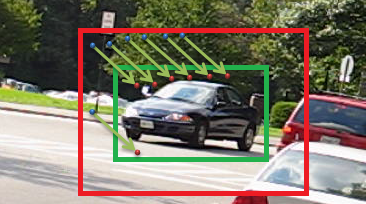
\includegraphics[height=0.285\textheight]{../images/tracking_points.png}
      \caption{Example image of points entering a tracking region (green) due to object motion in a video sequence.}
      \label{figurelabel_entering}
   \end{figure}
\setlength{\belowcaptionskip}{-10pt}

   \begin{figure}[thpb]
      \centering
      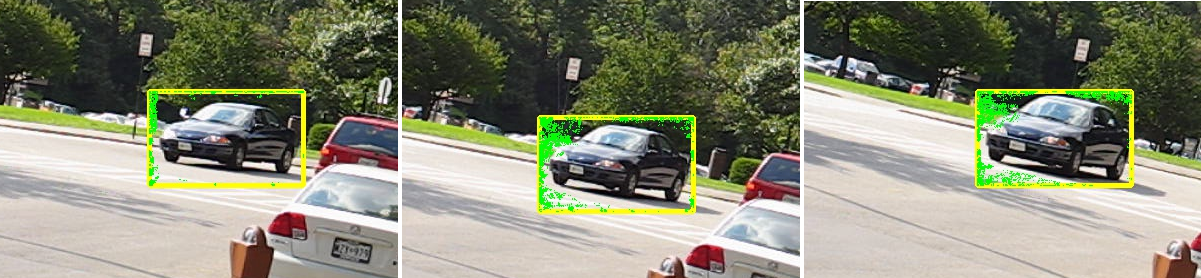
\includegraphics[width=1\textwidth]{../images/pointTr.png}
      \caption{Point tracking using an optical flow method.}
      \label{pointtr}
   \end{figure}


This idea can be applied in several levels in a video sequence. The first method to develop such an algorithm is to do it in the pixel level. The Fig. \ref{pointtr} shows some results by applying 
a dense optical flow technique (Fast Block Matching) in an external window. However, as it can appreciated, the results are rather sparse and after some time, the regularization of the 
optical flow method leads to some of the points being wrongly tracked inside the object boundaries. Both problems, sparsity and tracking errors due to drift and regularization, can be 
overcome by implementing the same idea, but in the superpixel level.
To save computational power, the tracked superpixels are 
limited to the ones that fall inside a control region (red box in the Fig.  \ref{figurelabel_entering}). 

Normally, after several frames, 
the labelled superpixels will almost completely cover the unwanted areas in a dynamic scene. We call this process background segments tracking and the process is summarized in the 
Algorithm \ref{algo1}.  The Fig. \ref{figurelabel_spflow} shows this idea in a real scenario. From left to right, initially the superpixels with 
elements outside the bounding box are labelled as background (green), then, as the sequence changes, the labelled superpixels flow inside the window, giving hints for the model initialization in the background-foreground separation algorithm.

\begin{algorithm}[ht]
\caption{Background regions tracking between a frames A and B}
\label{algo1}
\begin{algorithmic}
\REQUIRE list: $superpixelsA, superpixelsB$, rect: $trackerA, trackerB$, vector: $prev\_labels$

\STATE vector: $new\_labels$
\STATE $computeSuperPixelFlow()$
\FORALL{$superpixel \in superpixelsA$}
    \STATE $matches[superpixel] = getMatchesFromFlow(superpixel)$

	\COMMENT{ Check is previously labelled superpixels fall inside $trackerB$ }
	\IF{$superpixel \in prev\_labels$}
		\STATE $matchAB = superpixelsB[ matches[superpixel] ]$
    		\IF{$matchAB \in trackerB$} 
    			\STATE $new\_labels.push\_back( matchAB )$
    		\ENDIF
	\ENDIF 

	\COMMENT{ Check is new labelled superpixels fall inside $trackerB$ }    
    \IF{$superpixel \notin trackerA$} 
    	    \STATE $matchAB = superpixelsB[ matches[superpixel] ]$
    		\IF{$matchAB \in trackerB$} 
    			\STATE $new\_labels.push\_back( matchAB )$
    		\ENDIF
    	\ENDIF
\ENDFOR

\RETURN $new\_labels$
\end{algorithmic}
\end{algorithm}

At this point, some generic segmentation technique can be connected to the pipeline to refine the segmentation (e.g. region growing). However, graph based segmentation methods are preferred (\cite{c18}\cite{c15}) because the usual user interaction can be replaced by the tracked background regions, and the algorithms are faster and more robust.

   \begin{figure}[thpb]
      \centering
      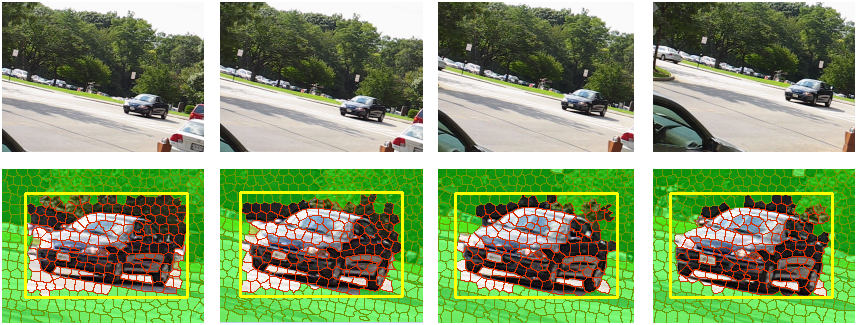
\includegraphics[width=1\textwidth]{../images/suppixflow2.png}
      \caption{Background segments automatic labelling and propagation, the flow goes from left to right.}
      \label{figurelabel_spflow}
   \end{figure}

\subsection{Segmentation results}

Fig. \ref{figurelabel_walking} shows the results for an image sequence where the interest object is the head of a person.
The head tracker and the superpixel flow provide information for better background-foreground separation. The
background-foreground models are updated as the frames go on, giving more robustness for sequential
propagation of the segmentation. The method is tested in the Walking Couple sequence, by allowing only a small amount of iterations in the
graph based segmentation. Observe how the contour in the man's head is correctly delineated when
another person's head occludes part of it. In this case, the superpixels that belong to the woman’s face
were correctly propagated and thus, labelled as background. Its also impressive that the segmentation process recovers after a heavy occlusion.
In this case, the fact that the tracker is also robust to the occlusion is a key factor that help the system maintain a correct segmentation through such a difficult 
case.

   \begin{figure}[thpb]
      \centering
      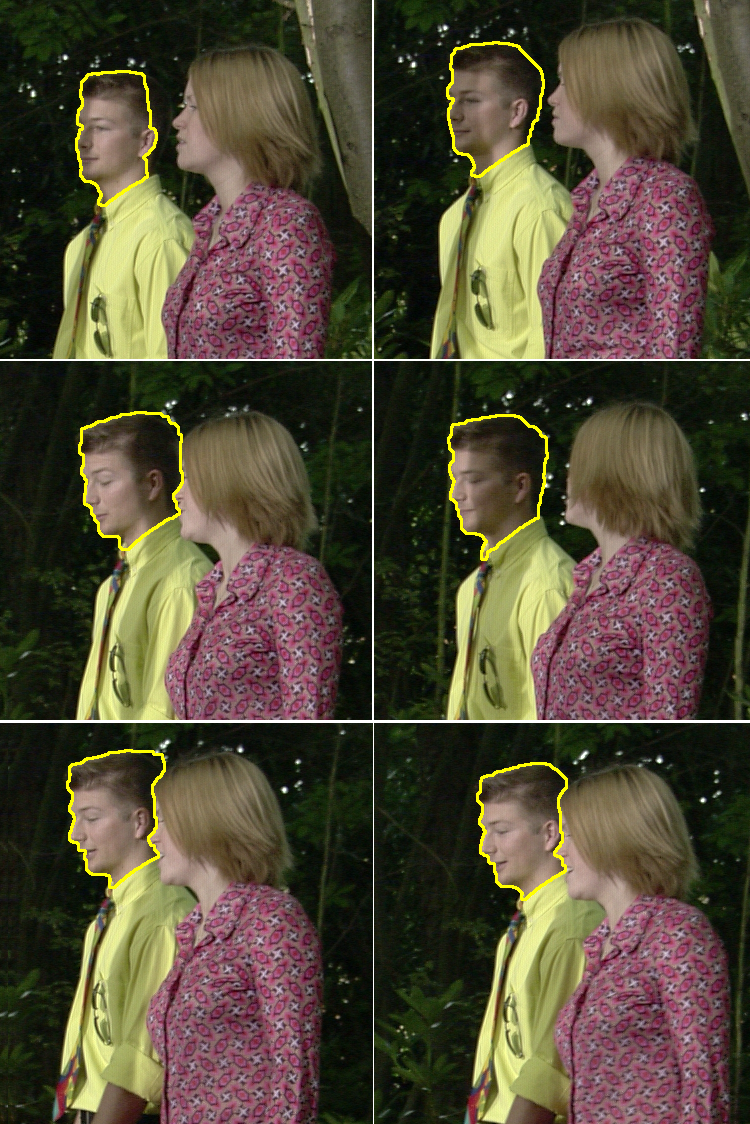
\includegraphics[width=1.0\textwidth]{../images/Sequence.png}
      \caption{Segmentation through the sequence “Walking
	       Couple” (Yellow contour) initialized in the man’s head. The yellow box correspond to the tracker output.
	        The labelled background superpixel are not shown for clarity.}
      \label{figurelabel_walking}
   \end{figure}

In order to understand the effect of including superpixel propagation in a video sequence for object
segmentation, some results are shown in the Fig. \ref{figurelabel_comp}. For these experiments only one iteration is
allowed in the graph-cut based methods. The top row frames (Fig. \ref{figurelabel_comp}) were initialized only with the tracker, 
and the bottom row was initialized with the superpixel tracking technique. 
Observe that in general, the contour delineated is usually better in terms of precision and
stability for the later one. Complete segmentation results can be observed in the Appendix \ref{app:seg}.

   \begin{figure}[thp]
      \centering
      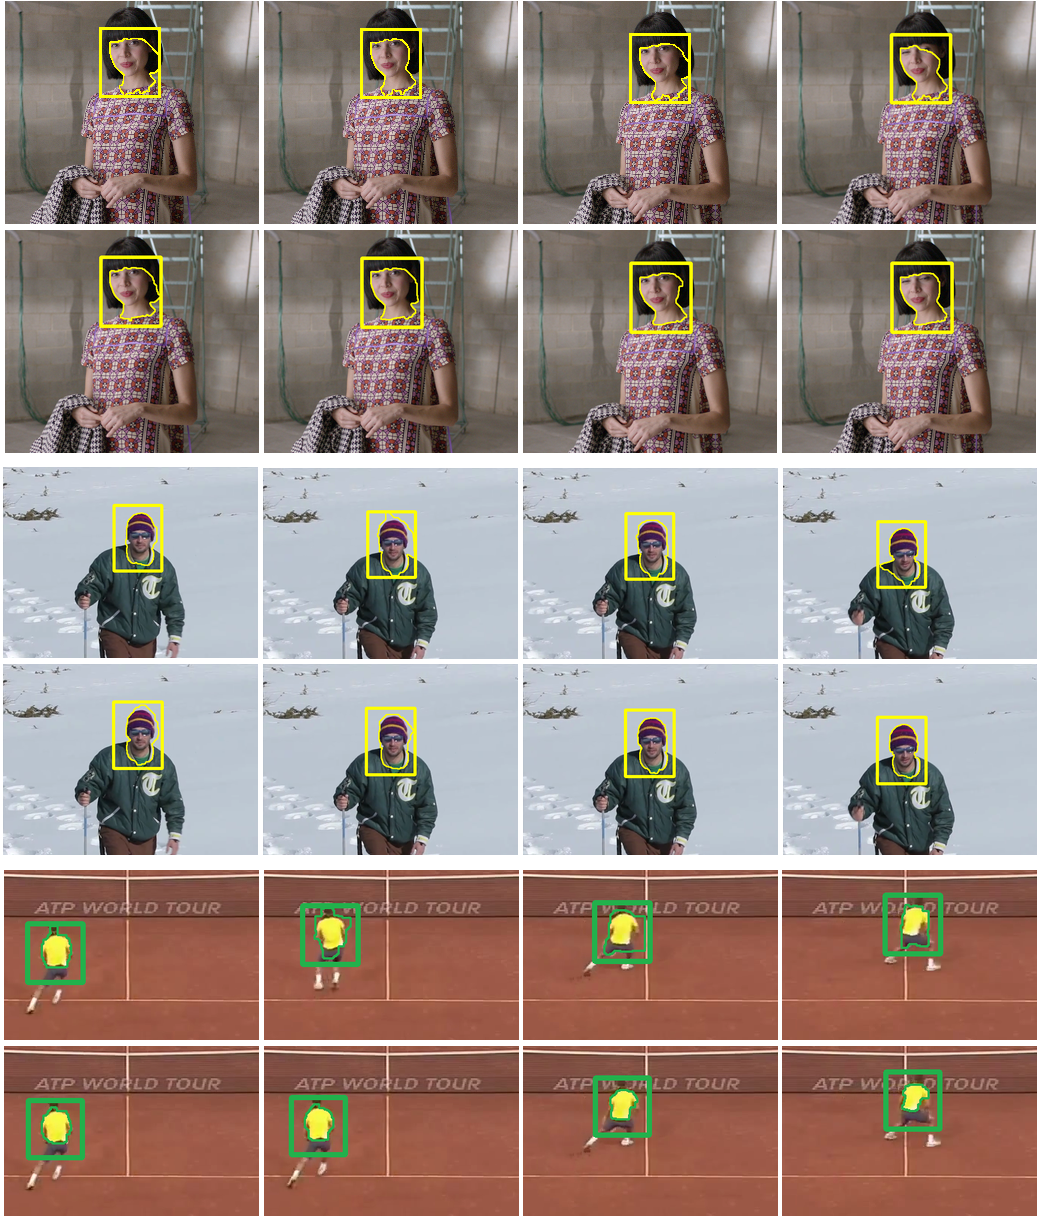
\includegraphics[width=1.0\textwidth]{../images/compareSegm.png}
      \caption{Face segmentation in the “Amelie Retro” and the
	      “Snow shoes” sequences in several different frames, and T-shirt extraction from Tennis sequence. For each
	       group, the Top Row: One-iteration window-based graph-cuts;
	       and the Bottom Row: One-iteration graph-cuts initialized with superpixel tracking.}
      \label{figurelabel_comp}
   \end{figure}

\section{Flow estimation}
%\subsection{Flow estimation}
\label{sec:core}

The object flow consist on computing the motion field for an object of interest through an image
sequence. The most usual approach to solve a problem like this is to implement some of the available
optical flow techniques through the complete sequence and perform the flow integration. 
However, this process results in high levels of motion drift \cite{c18}\cite{c19} and usually the motion of the interest
object is affected by a global regularization. In some extreme cases, the interest object motion
may be totally blurred and other techniques have to be incorporated. Moreover, the diversity
of natural video sequences makes difficult the choice of one optical flow technique over another, even when specialized
databases are at hand \cite{c17}, because currently no single method can achieve a strong 
performance in every of the available datasets. Most of these methods consist in the minimization 
of an energy function with two terms (As was previously mentioned in the Sec. \ref{chap:intro}). The data
term is mostly shared between different approaches, but the prior or spatial term is different, and basically states 
under what conditions the optical flow smoothness should be maintained or not. In a global approach, however,
this is a difficult concept to define. Most of these smoothness terms rely in appearance differences or gradients.
All these meaning that, unavoidably, some methods may be more reliable for some cases but weaker for others. 
It can be argued that this behaviour may be caused because most of the techniques do not count with a way to identify 
firmly where exactly this smoothness prior can be applied. 

It is difficult, nevertheless, to blame the authors for the choice of some regularization 
terms, since the more robust the regularization terms is, and the higher level knowledge is applied, the more difficult is to minimize the 
energy function, and thus, the more difficult is to obtain a reliable global solution. 
The modern advances in non-convex optimization methods have allowed some authors 
to go further in the writing of these energy functions, but at the end they still rely in the pixel level to determine whether a strong regularization 
should be applied to a zone or not.


   \begin{figure}[thpb]
      \centering
      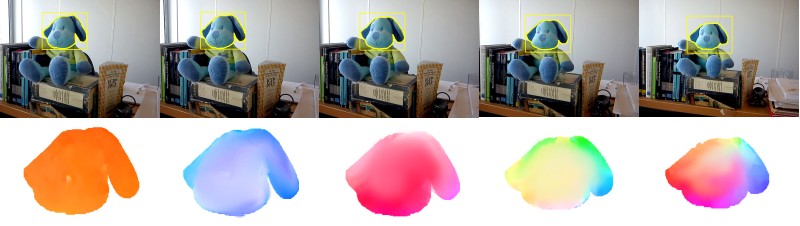
\includegraphics[width=1.0\textwidth]{../images/objectflow.png}
      \caption{Object flow with the color code of \cite{c17} (bottom) for frames in the Puppy sequence (up). }
      \label{of}
   \end{figure}

The main idea behind the object flow is that given the availability of several robust tracking techniques, and the proposed
segmentation method for video, the optical flow computation can be refined by computing it successively between pairs
of tracked windows. The basic proposal to perform this refinement consist on considering the segmentation limits  as reliable smoothness boundaries. 
This is, of course, under the assumption that the motion is indeed smooth within the object region. 
This is assumption is not far from reality in most scenes with an interest object, and it is indeed a better way to determine the limits of the regularization 
than using the difference between raw pixel values.
Naturally, as the object tracker is included, is expected that the object flow should be more robust to rapid motions than the
optical flow. 
Thus, the full motion is split in two, the long range motion, given by the tracker window, and the precision part, given by the targeted optical flow. The Fig. \ref{of} shows 
the object flow for a frame in the Puppy sequence. Observe the motion vectors are computed only inside the object of interest, preserving a strong smoothing prior, but 
also allowing internal variations in the flow. 

As a first approximation to the object flow, the Simple Flow technique \cite{c21} is taken as core base. This is because of its scalability 
to higher resolutions and because its specialization to the concept of object flow is only natural. The reason behind this is that in the Simple Flow pipeline 
the smoothness localization can be easily specified through computation masks. More specifically, the initial computation mask is derived from 
the segmentation performed as prior step. An iterative multi-scale approach based on this initialization follows. The original method uses bilateral filtering to refine each flow result. 
However, as a reliable segmentation mask is provided, this bilateral filtering is replaced by a Gaussian filter applied within the limits of this mask, highly improving the speed of the 
flow estimation. 

   \begin{figure}[thpb]
      \centering
      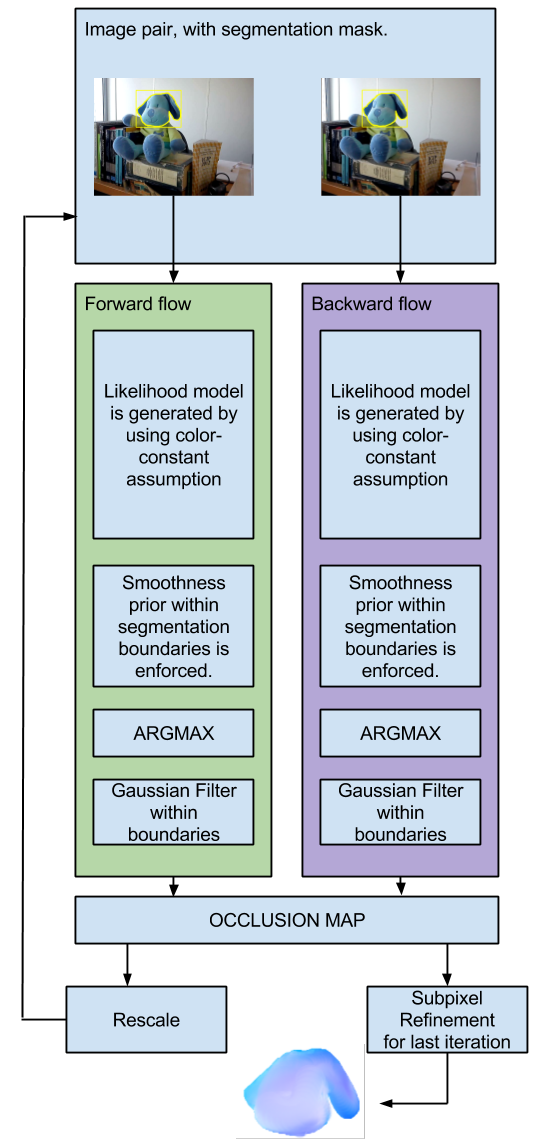
\includegraphics[height=1.0\textheight]{../images/simpleobjectflow.png}
      \caption{ Simple object flow algorithm diagram.}
      \label{sof_d}
   \end{figure}

In more detail, 
for every pixel within the segmentation boundaries a vector $e$ of dimension $n^2$ is computed 
by extracting a color difference $n$x$n$ window centred in that pixel. The energy $E$ (as in \ref{eq_simple}) is computed 
within the 
segmentation boundaries 
by applying a bilateral filter, 
using the color data of the initial 
frame to define the filter weights. 
The flow for the given pixel is the vector that minimizes $E$. The final bilateral filter applied over the computed flow field for every scale is replaced by a Gaussian filter limited by the segmentation masks. The process is done twice, from $I_t$ to $I_{t+1}$ and vice-versa. 
An occlusion mask is generated by eliminating the flows that do not correspond with its 
backward counterpart ($||(u_f,v_f)-(-u_b,-v_b)||$ is too high). The process is repeated in 
several scales to account for possible large motions inside the studied object (Fig. \ref{sof_d}).

However, direct modifications in other optical flow methods can be further studied. For instance, in graph-cut based 
minimization approaches, the regularity constraints can be precisely targeted by disconnecting foreground pixels from background ones.

   \begin{figure}[thpb]
      \centering
      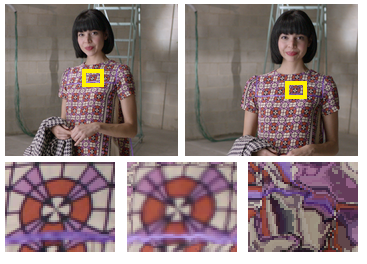
\includegraphics[width=0.66\textwidth]{../images/objectflow_nosegm.png}
      \caption{Top row: First and last frames used from the Amelia sequence. Bottom row: From left to right: Groundtruth patch; patch generated with the 
basic object flow combining the {\it Struck} Tracker and the {\it TVL1} optical flow; and patch generated with the globally computed  {\it TVL1} optical flow.}
      \label{of_nose}
   \end{figure}

The object flow concept is valid, however, for those cases where there is not a separable object, and the segmentation is not valid or possible to extract. 
In order to show this and the fact that only combining the tracker information with a locally computed optical flow is already an improvement to a global 
optical flow, the Fig. \ref{of_nose} shows an experiment where a patch from a dress is extrapolated by using the most basic object flow definition (no segmentation) 
and by a globally computed optical flow. It can be seen that the results are better for the first method.




\section{Feedback for tracking methods} \label{sec:feedback}

As previously shown in the Fig. \ref{figurelabel_sys} the acquired knowledge by the segmentation mask, and flow estimation can be used to 
feedback the tracker method, and generate a more precise position of the object in the next frame. There are several ways to perform this feedback 
depending on the specific tracking method used. However, to mantain certain generality in the pipeline of the object flow, the used cues are the ones 
given by the segmentation mask and the tracked background regions that could behave as occlusions. 
In the most of the tracking by detection methods, a sampling step (which can be explicit like in the {\it MIL} tracker, or implicit, 
like in the {\it Struck} tracker) is performed to extract features that are valid as possible to represent the target object. 

   \begin{figure}[thpb]
      \centering
      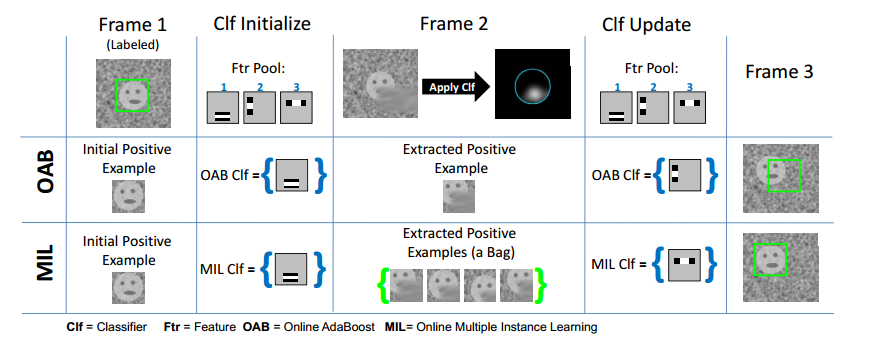
\includegraphics[width=0.95\textwidth]{../images/mil.png}
      \caption{An overview on how tracking-by-detection methods try to deal with occlusions. Extracted from \cite{c25}.}
      \label{tr_mil}
   \end{figure}
   
When occlusions happen, the most of the methods have a hard time to select a correct bag of features to represent the said object, as it gets difficult 
for the learning method to explain the object after and before occlusions with a given set of features. The Fig. \ref{tr_mil} shows how Online Adaboost 
and Online Multiple Instance Learning try to deal with this problem when a small occlusion happens.

Frame 1: Consider a simple case where the classifier is allowed
to only pick one feature from the pool. One positive patch and several negative patches  are extracted, and 
the classifiers are initialized. Both OAB and MIL result in identical classifiers - both choose feature no.1 because it responds well with the mouth of
the face. Frame 2: The mouth is now occluded, and the classifier trained in the previous step does not perform well. Thus, the most probable image patch is no
longer centered on the object. OAB uses just this patch to update; MIL uses this patch along with its neighbors. Frame 3: When updating, the classifiers try to pick the feature that best discriminates the current example as well
the ones previously seen. OAB has trouble with this because the current and previous positive examples are too different. It chooses a bad feature.
MIL behaves better in this case because a correct sample was included in the positive bag \cite{c25}. This may not be the situation for heavier oclussions, where the chances of taking the object as sample are low or null. In these cases, having a precomputed occlusion mask of the last frame, 
can help to select better which features to take into account, or even to avoid completely the sampling process in a given frame. 

   \begin{figure}[thpb]
      \centering
      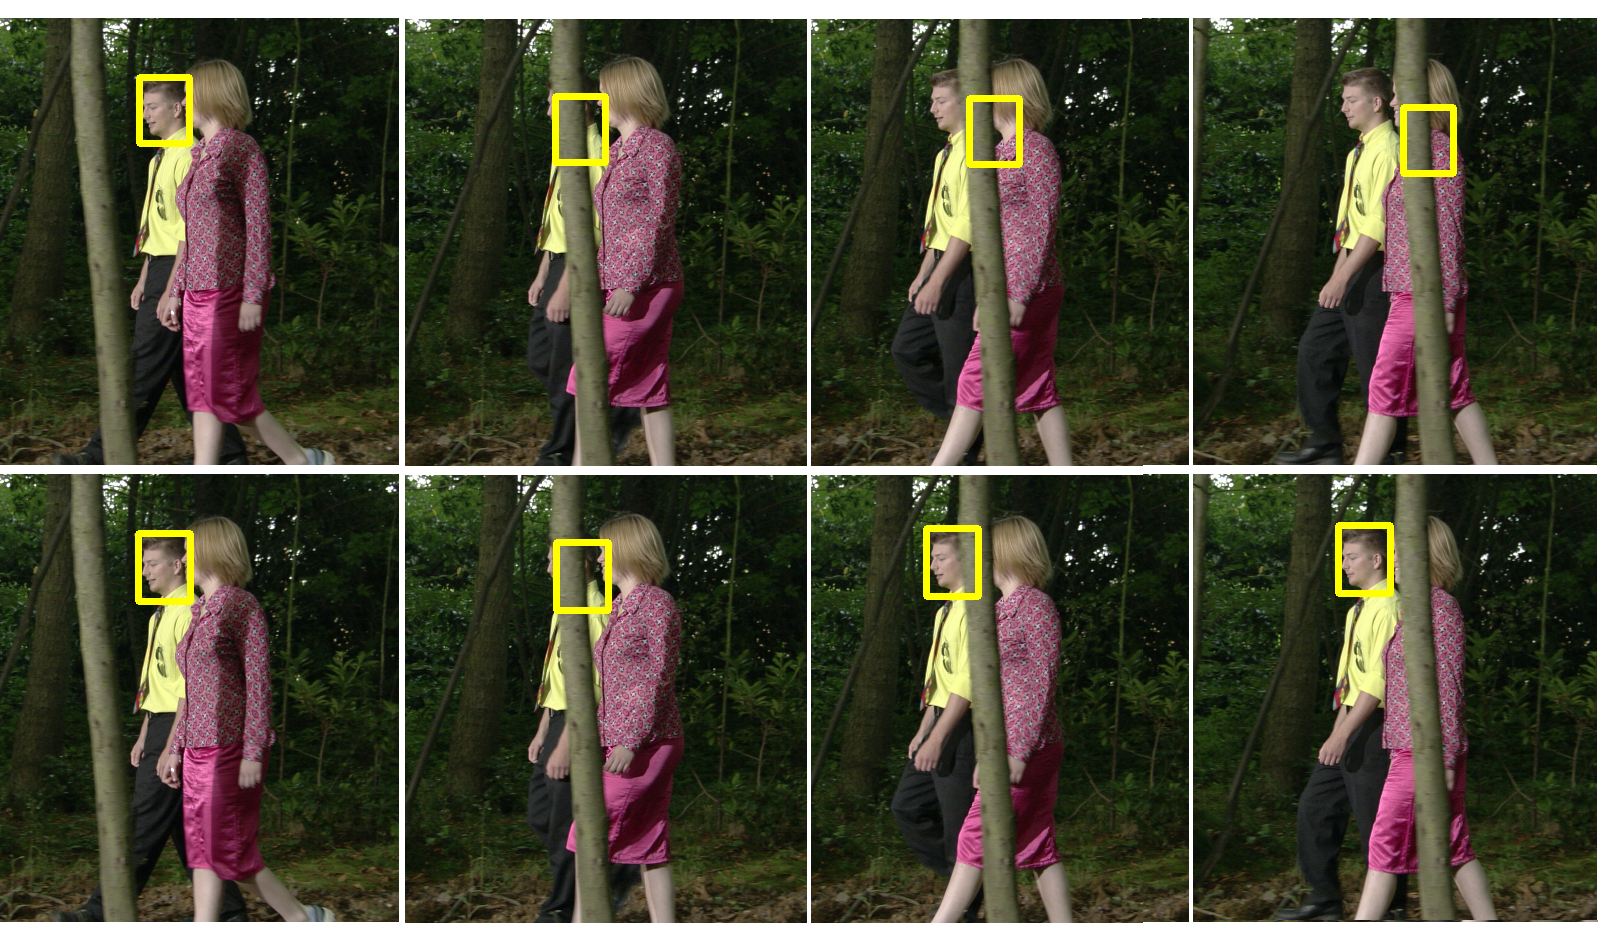
\includegraphics[width=1.0\textwidth]{../images/struckComp.png}
      \caption{Struck tracker in the Walking Couple sequence. Top: Original Implementation. Bottom: Struck tracker with sampling refinement by background regions tracking.}
      \label{tr_strucktest}
   \end{figure}
   
This idea is summarized with the experiment performed with the {\it Struck} tracker. These results can be observed in the Fig. \ref{tr_strucktest}. The sampling process is altered to receive feedback 
from the background segmentation. As it can be seen, for the top row (original implementation using only Haar features) the tracker starts 
learning the tree (oclussion object) since the third shown frame. In the other hand, as the sampling process is modified by rejecting the zones 
labelled as background (including the tree), the tracker quickly recovers after the oclussion in the bottom row. Both experiments were performed 
with a very narrow search window, and by using only Haar features. This is, the tracker did not learn the features extracted 
from the occluding object, and the original object is recaptured when it reappears in the scene. Altough these experimentes are promising, a more deep study is needed, since the {\it Struck} tracker can be more robust if an optimal search window is used, and more features are included in 
the machine learning process.

